\section{Introduction} 

This document contains the course notes for the mechanism design exercise. Mechanisms are a vital part of engineering systems and can provide significant gains in the performance and effectiveness of products. The aim of this exercise is to give you an appreciation of the challenges in designing a mechanism. We will also be situating ourselves in the early design phases of~\citet{pahl2013} systematic approach to Engineering Design (\cref{fig-design-process}). This differentiates this exercise from the shaft design where we focused on the stages associated with the detailed design phase.

\begin{figure}
  \centering
  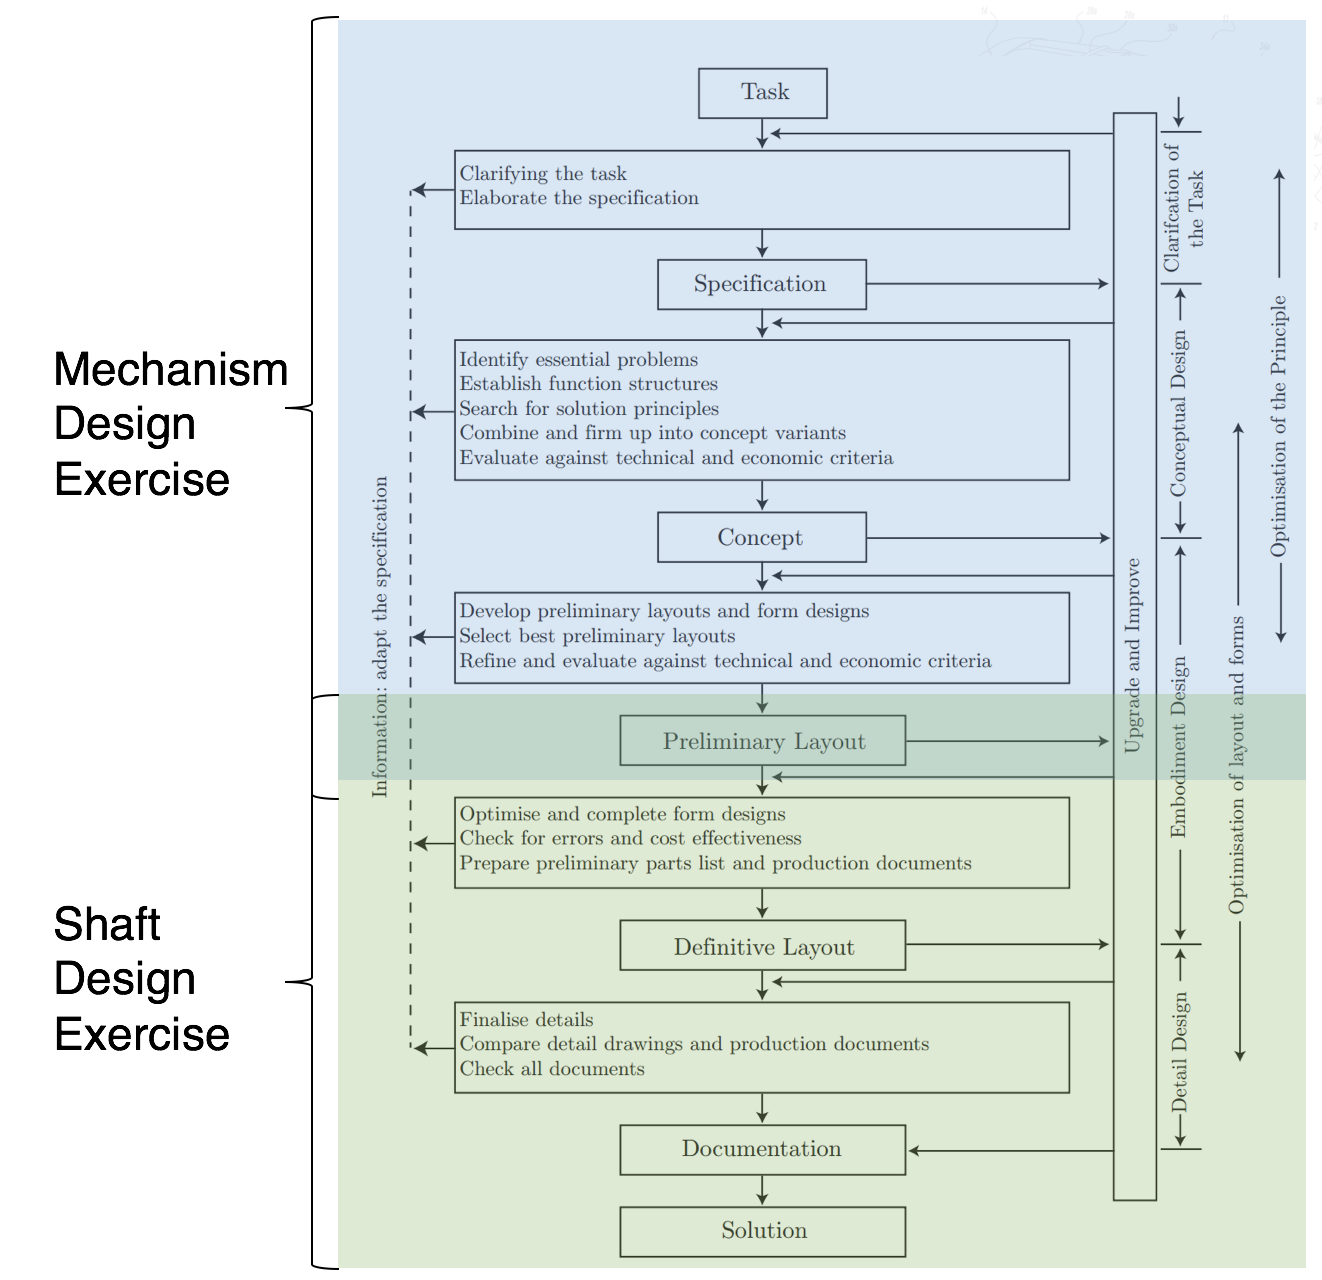
\includegraphics[width=0.9\textwidth]{figs/design-process.png}
  \caption[Aligning ourselves to the Systematic Design Process model]{Aligning ourselves to the Systematic Design Process model~\citep{pahl2013}}
  \label{fig-design-process}
\end{figure}

Although there is enough information provided in these notes to complete the course, you should be researching and reading further material to support the your design decisions.

\marginnote{Intended Learning Outcomes} The intended learning outcomes are as follows:

\begin{enumerate}
  \item Provide awareness of mechanisms and their applications
  \item Practice design thinking, rationale capture and build on the feedback from the shaft design
  \item Apply system modelling tools to preliminary design scenarios
  \item Generate feasible mechanism layouts for the design task
  \item Practice your theoretical engineering knowledge in an unconstrained and unfamiliar context
\end{enumerate}

\marginnote{Engineering Skills/Software} Over the next six weeks, you will be applying and further developing your engineering skill-set. Some of the key skills you will be using are:

\begin{multicols}{2}
\begin{itemize}
\item Problem definition
\item Systems modelling
\item Concept generation
\item Concept selection
\item Initial calculations
\item Selection design
\item Prototyping
\item Kinematics
\item Damping
\item Motors
\item Gearing
\item \LaTeX
\item Simulink
\item Linkage Modeller
\end{itemize}
\end{multicols}

Each\marginnote{Industry} year, we have an Industrial Advisory Board meeting to discuss the Engineering programme. This is where industry can raise ideas and features that they would like to see in the course. Here are a selection of quotes that provide some of the industrial rationale for the mechanism design exercise.


\begin{center}
``We want students to have a multi-disciplinary skill-set and can apply advanced design analysis tools in real-world scenarios.'' \\~\\
``We have been doing hand-calculations for 30-years and have been able to make some great products but we need new engineers who are able to to do both so that we move beyond what we currently do.''
\end{center}

In\marginnote{Student} addition to the industrial feedback, we look at past student feedback to see how we can improve the delivery of the course to best support the intended learning outcomes. This is one of the reasons this document now exists! Past student feedback wanted a single source of core course material that they could refer to and keep as a memento of the exercise!

Here's some quotes from the previous years:

\begin{center}
``This exercise pushed my knowledge of engineering systems and taught me new tools to use'' \\~\\
``This exercise was tough but as long as you keep up with the lectures and tasks then you will learn a hell of a lot''\\~\\
``Recommendations for next years students, WRITE UP AS YOU GO ALONG! Don't stress yourselves out by leaving it to the last minute''\\~\\
``I did not see the point of trying \LaTeX{} and Simulink but now I realise it’s another tool to help me. Good to put on the C.V.''\\~\\
``Hard work and had differing opinions from the lecturers. It was only when I read the feedback that I realised it was all about describing the process and providing the rationale behind what I have done.''
\end{center}

The exercise has been deliberately set to push the boundaries of your engineering knowledge and skills, and if you attend all the lectures and tutorials then there should be no reason for you not to be able to attain a 1st in your studies.

\section{Multi-Bar Mechanisms}

Mechanisms\marginnote{Applications} are a fundamental part of engineering products and have been used to solve many engineering design problems. Some of the key applications involve: 

\begin{itemize}
  \item The translation of motion \& forces;
  \item Improving the performance of a product;
  \item Simplifying the control system of a product;
  \item Increasing the efficiency of a product; and,
  \item Deploying a product.
\end{itemize}

One\marginnote{Translation of Motion and Forces} of the primary applications of mechanisms is to translate motions and forces. For example, pistons turn the explosive energy of combustion from a linear motion to a rotational motion. Window hinges help to extend the window, which may be outside the normal reach of a human, and vice grips use mechanisms to gain mechanical advantage, which increases the force being applied by a human.

Using\marginnote{Improve the Performance of a Product} mechanisms to gain a mechanical advantage is also one method of increasing the performance of a product. Multi-bar mechanisms are also widely applied in suspension geometry. For example, double wishbone suspension (\cref{fig-double-wishbone}) is -- in effect -- a four-bar mechanism, which provides designers the ability to customise the toe, camber and caster angles of a car wheels geometry. 

%https://i.pinimg.com/originals/3b/76/6f/3b766f731012a32538bb121e380e943d.png
\begin{marginfigure}[-1em]
  \centering
  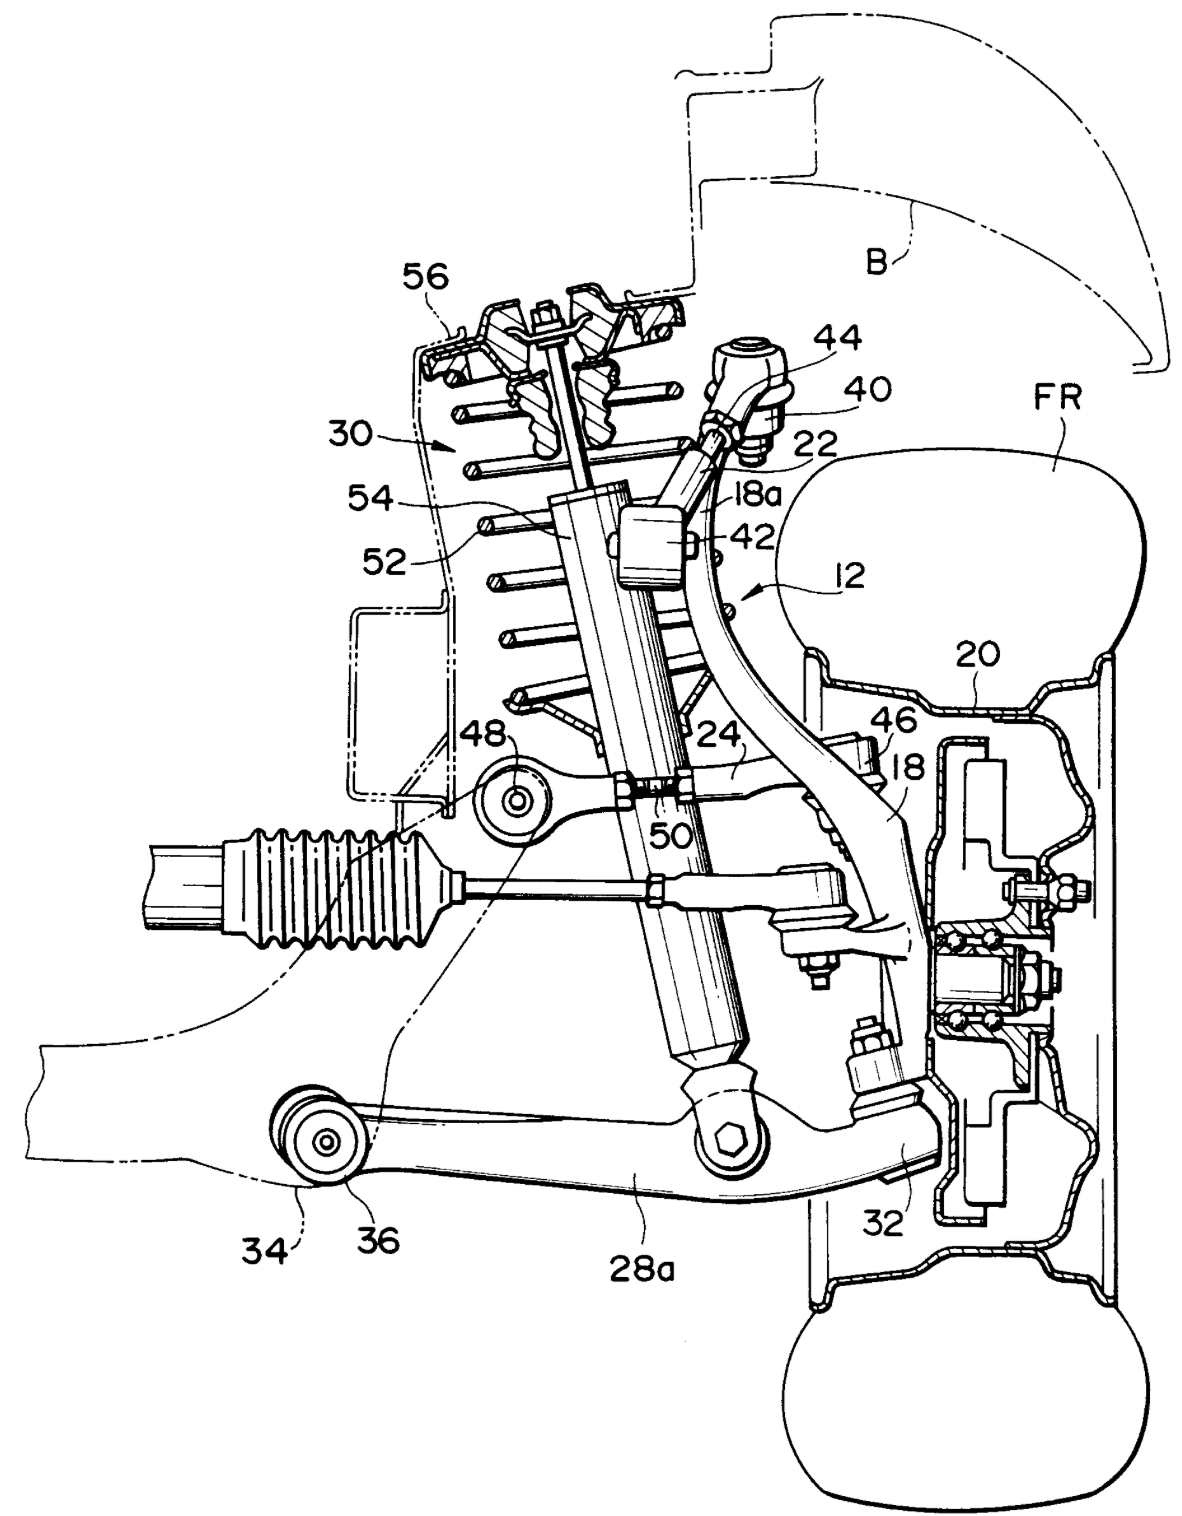
\includegraphics[width=0.5\textwidth]{figs/DoubleWishbone.png}
  \caption{Double wishbone suspension}
  \label{fig-double-wishbone}
\end{marginfigure}

The double wishbone also provides dynamic performance gains by automatically increasing the negative camber gain when the suspension is being compressed. This further supports the wheel/road contact, helping the car corner more effectively.

With\marginnote{Simplify the Control System of a Product} the rise of low-cost micro-controllers and electronic servo systems, many designs can easily fall into the trap of leaving the control of products to the development of advanced control software. However, if designed right, a mechanism can significantly reduce the workload of a control system by providing the intended motion through the geometry alone.


Level-luffing cranes is one such example (\cref{fig-level-luffing}). This cranes mechanisms has been designed to ensure that a cargo's height is maintained whilst being moved in and out by the crane. This significantly reduces the level of cargo sway, which competing manufacturers have to overcome with advanced electronic control systems. 

% http://www.kranunion.de/typo3temp/cokcb2web/files/e16d6cad9298bde4320172e05d07faea/Kondor4c.jpg
\begin{marginfigure}[-10em]
  \centering
  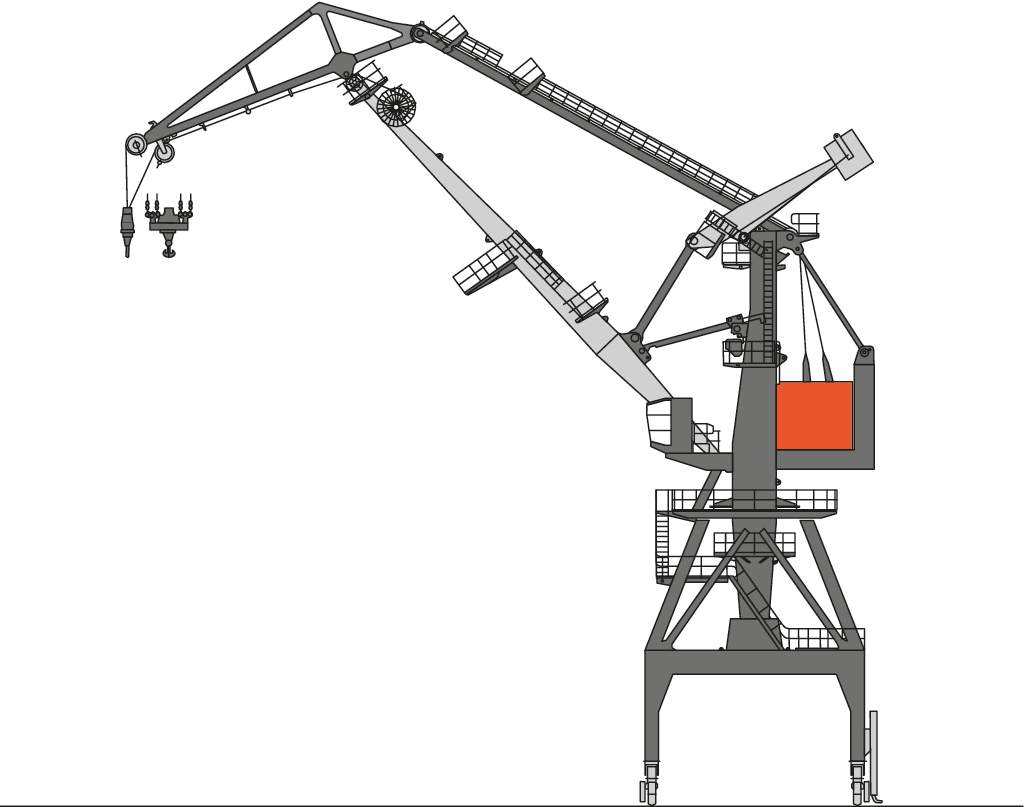
\includegraphics[width=\textwidth]{figs/Kondor4c.jpg}
  \caption{Level-luffing crane}
  \label{fig-level-luffing}
\end{marginfigure}

\marginnote{Deploy a Product} One of the other areas where mechanisms are used is in the deployment of products. Scissor jacks, convertible roofs and satellite solar panels (\cref{fig-solar}) are all examples where multi-bar mechanisms are used to deploy and retract a product. In the case of a satellite, the deployment of the solar array has to be carefully calculated as the residual forces can lead to waves of energy be propagated along the solar panel and forces that can lead to the satellite going off course.

%http://patentimages.storage.googleapis.com/US20140263847A1/US20140263847A1-20140918-D00008.png
\begin{marginfigure}
  \centering
  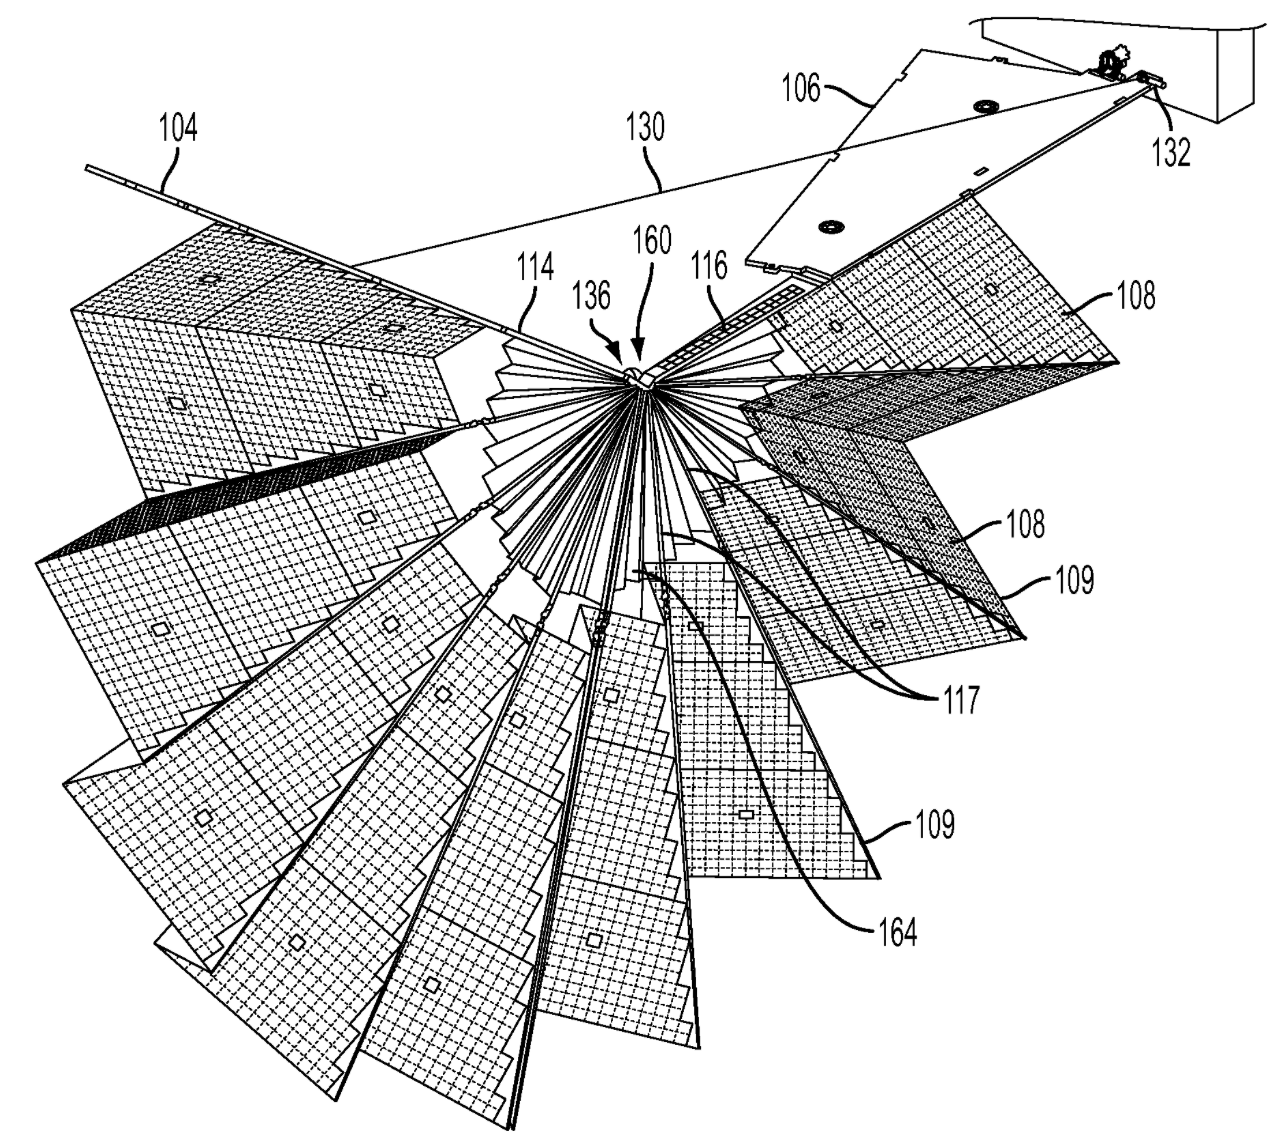
\includegraphics[width=\textwidth]{figs/solar-arrays.png}
  \caption{Solar array deployment}
  \label{fig-solar}
\end{marginfigure}


Mechanisms\marginnote{And Art!}  have also found themselves into art with Theo Jansen using multi-bar mechanisms to develop strand beasts (\cref{fig-strand}). These beasts can be found walking the beaches of the Netherlands and use mechanisms to translate power of wind into motion along the shore-side.

% https://media.newyorker.com/photos/59096853019dfc3494ea0fa5/master/w_727,c_limit/110905_r21202_g2048.jpg
\begin{figure}[h!]
  \centering
  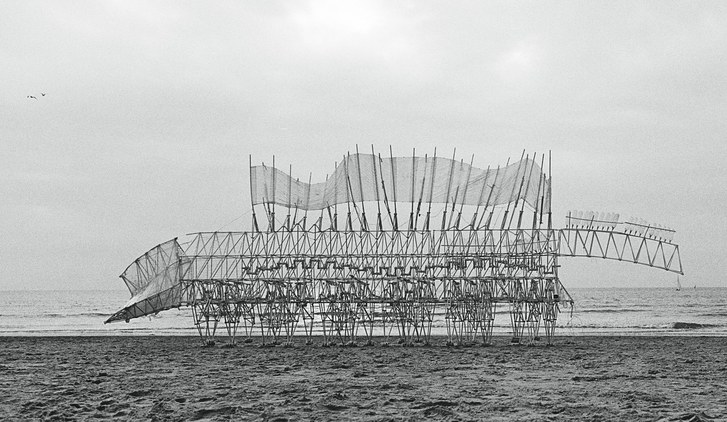
\includegraphics[width=0.8\textwidth]{figs/strand-beast.jpg}
  \caption{Strand beasts}
  \label{fig-strand}
\end{figure}

Mechanism\marginnote{Research at the University of Bath} development are also features in the research at the University of Bath. Previous research has developed tools such as the Constraint Based Modeller, which supports the design of mechanisms by providing potential mechanism solutions that can achieve a desired motion path whilst also being fixed at certain positions and/or have maximum number of beams that can be used~\cite{edmunds2011}. You will be introduced to these tools in your 3rd and/or 4th years of study.

Current research is focused on the evaluation of six-bar spherical mechanisms and the motion profile behaviour (\cref{fig-spherical}). These are notoriously difficult to construct and are highly-sensitive to perturbations and changes to the lengths of the beams. In fact, the motion of the jaw chewing can be approximated by these mechanisms. Developing mechanisms that can mimic this behaviour have been used in studies into the delivery of oral medication.

\begin{figure}[ht!]
  \centering
  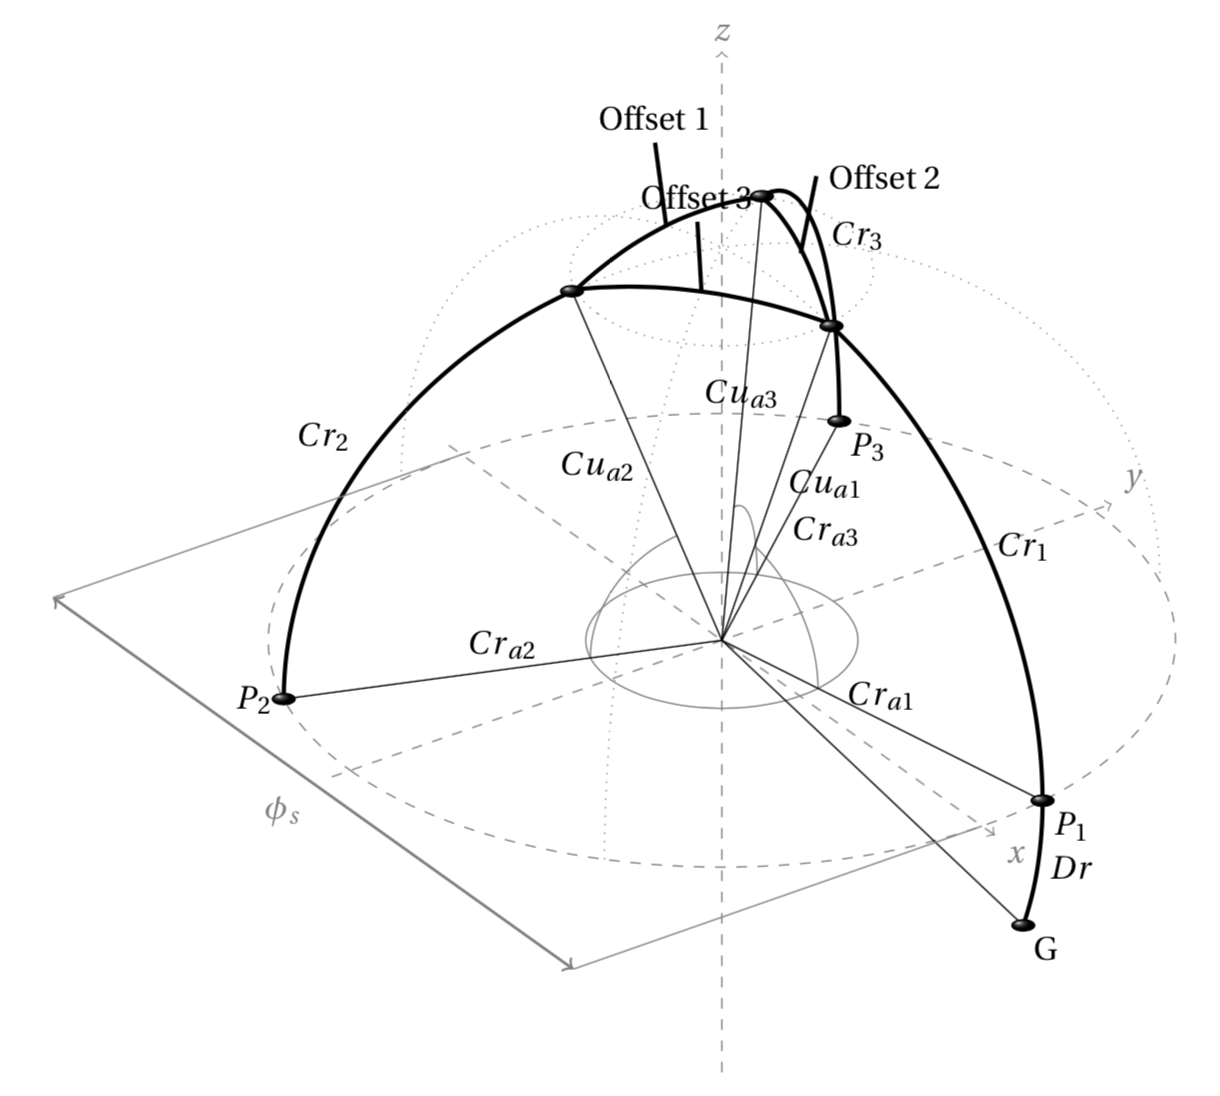
\includegraphics[width=\textwidth]{figs/spherical-bar.png}
  \caption{Spherical bar mechanism}
  \label{fig-spherical}
\end{figure}
